\chapter{Testing}

\section{Test plan}

\subsection{frmLoginForm, frmMainMenu, frmAdd, frmRemove, frmList}

I will test whether each form displays and each of its buttons and drop down boxes work, and that the user's input validates, if applicable.

\subsection{frmReportLog, frmReportQuote, frmReportInvoice, frmReportSurvey, and other reporting forms}

I will test whether each form displays and the buttons and drop down menus work, and the opening of the various documents, if applicable.

\section{Test data tables}

\subsection{Data entry and validation test data}

\begin{longtable}{ | p{4cm} | p{4cm} | p{4cm} | }
	\hline
	\textbf{\textcolor{red}{ERRONEOUS DATA}} & \textbf{\textcolor{blue}{BOUNDARY DATA}} & \textbf{\textcolor{black}{NORMAL DATA}}\\
	\hline
\end{longtable}

(The \textbf{NORMAL} test data is black to save colours such as green blinding the reader.)

\subsubsection{frmLoginForm}

\begin{longtable}{ | p{5cm} | p{5cm} | }
	\hline
	\textbf{Username} & \textbf{Password}\\
	\endfirsthead
	\hline
	Username (cont.) & Password (cont.)\\
	\endhead
	\hline
	sfs & sfs\\
	\hline
	sfs & \textcolor{blue}{sfss}\\
	\hline
	\textcolor{red}{NULL} & \textcolor{red}{NULL}\\
	\hline
\end{longtable}

\subsubsection{frmAddCustomer}

\begin{longtable}{ | p{1cm} | p{1.5cm} | p{1.5cm} | p{1cm} | p{1.5cm} | p{1cm} | p{1cm} | p{1cm} | p{1.5cm} | p{2.6cm} | }
	\hline
	\textbf{Title} & \textbf{Name} & \textbf{Bill Addr.} & \textbf{Bill Post.} & \textbf{Inst. Addr.} & \textbf{Inst. Post.} & \textbf{Home Tel. No.} & \textbf{Mob Tel. No.} & \textbf{Email Addr.} & \textbf{MPAN No.}\\
	\endfirsthead
	\hline
	\textbf{Title (cont.)} & \textbf{Name (cont.)} & \textbf{Bill. Addr. (cont.)} & \textbf{Bill Post. (cont.)} & \textbf{Inst. Addr. (cont.)} & \textbf{Inst. Post. (cont.)} & \textbf{Home Tel. No. (cont.)} & \textbf{Mob. Tel. No. (cont.)} & \textbf{Email Addr. (cont.)} & \textbf{MPAN No. (cont.)}\\
	\endhead
	\hline
	Mr. & David Ken & Flat 4R, York Way, London & N1 & Bill. Addr. & Bill. Post. & 020 564 8374 & 07284 839284 & davidken @ hotmail . com & 49573948384434\\
	\hline
	Mr. & Joe Bloggs & BloggLand & BL06 G55 & Limey & LI20 8ED & 01238 938439 & NULL & joe @ me . com & 35739384923998\\
	\hline
	& & & & & & & & & \textcolor{red}{123456789012345}\\
	\hline
	& & & & & & & & \textcolor{red}{hi.me.uk} &\\
	\hline
\end{longtable}

\subsubsection{frmAddSupplier}

\begin{longtable}{ | p{3cm} | p{4cm} | p{2cm} | p{4cm} | p{3cm} | }
	\hline
	\textbf{Name} & \textbf{Address} & \textbf{Postcode} & \textbf{Telephone Number} & \textbf{Contact name}\\
	\endfirsthead
	\hline
	\textbf{Name (cont.)} & \textbf{Address (cont.)} & \textbf{Postcode (cont.)} & \textbf{Telephone Number (cont.)} & \textbf{Contact name (cont.)}\\
	\endhead
	\hline
	Segen & Wesley Hall, Barrack Road, Aldershot & GU11 3NP & 01252 334412 & Ben\\
	\hline
\end{longtable}

\subsubsection{frmAddComponent}

\begin{longtable}{ | p{4cm} | p{3cm} | p{4cm} | p{2cm} | p{3cm} | }
	\hline
	\textbf{Name} & \textbf{Type} & \textbf{Serial Number} & \textbf{Panel kWp} & \textbf{Supplier}\\
	\endfirsthead
	\hline
	\textbf{Name (cont.)} & \textbf{Type (cont.)} & \textbf{Serial Number (cont.)} & \textbf{Panel kWp (cont.)} & \textbf{Supplier (cont.)}\\
	\endhead
	\hline
	Sharp ND-185R1S & Panel & n\slash a & 4 & Segen\\
	\hline
\end{longtable}

\subsection{Test data for displaying and removing data}

There are data removal\slash data display tests which have no test data apart from what I remove or the documents I open to display.  What I remove or display is detailed in the results table.

\section{Results of the tests}

\subsection{frmLoginForm tests}

\begin{longtable}{ | p{2cm} | p{4cm} | p{4cm} | p{4cm} | }
	\hline
	\textbf{Test number} & \textbf{Test details} & \textbf{Expected result} & \textbf{Actual result}\\
	\endfirsthead
	\hline
	\textbf{Test number (cont.)} & \textbf{Test details (cont.)} & \textbf{Expected result (cont.)} & \textbf{Actual result (cont.)}\\
	\endhead
	\hline
	1.1 & Click the cancel button to close the program from this form. & The cancel button ends the running program. & The cancel button ends the running program.\\
	\hline
	1.2 & The first row of the frmLoginForm test data table, so `sfs' and `sfs' as the username and password respectively. & Authentication successful; the menu form displays and the login form disappears without error. & Authentication successful; the menu form displays and the login form disappears without error.\\
	\hline
	1.3 & The second row of the first frmLoginForm test data table, so `sfs' and `sfss' as the username and password respectively.  The extra `s' in the password is deliberate, for testing purposes. & Authentication unsuccessful; an error message displays and the fields are blanked for the user to re-enter the details. & Authentication unsuccessful due to erroneous data; the error message displays.  See figure~\ref{fig:test_onedottwo} on page~\pageref{fig:test_onedottwo}.\\
	\hline
	1.4 & The third row of the first frmLoginForm test data, so `' and `' (empty (NULL) textboxes). & Rejected due to null data: error message the same as in the above test specified. & Rejected due to null data: error message the same as the above specified.\\
	\hline
	1.5 & Here I will test whether the OK button works. & As the above three tests have succeeded, it is guaranteed that the OK button works. & The OK button works.\\
	\hline
	1.6 & Testing that the main menu displays after having clicked OK, if there are no errors in the username and passwords. & The main menu displays and the login form hides itself. & The expected result is the final outcome.\\
	\hline
\end{longtable}

\subsection{frmMainMenu tests}

\begin{longtable}{ | p{2cm} | p{4cm} | p{4cm} | p{4cm} | }
	\hline
	\textbf{Test number} & \textbf{Test details} & \textbf{Expected result} & \textbf{Actual result}\\
	\endfirsthead
	\hline
	\textbf{Test number (cont.)} & \textbf{Test details (cont.)} & \textbf{Expected result (cont.)} & \textbf{Actual result (cont.)}\\
	\endhead
	\hline
	2.1 & A test of two forms, really, documented in frmLoginForm's test 1.6. & &\\
	\hline
	2.2 & Testing whether the Quit button quits the program. & At this stage, because the main menu is the main menu, it would make no sense to return the user to the login form as it would also cause problems with databases and authentication, so the program should close completely if this button is clicked. & The program closes completely.\\
	\hline
	2.3 & Testing whether the Add button displays `frmAdd'. & On click, the main menu hides and `frmAdd' appears. & Exactly that.\\
	\hline
	2.4 & Upon returning to the main menu, testing whether the Remove button works. & On click, the main menu hides itself and `frmRemove' appears. & What is expected to happen happens.\\
	\hline
	2.5 & Upon returning to the main menu, testing whether the List button works. & On click, the main menu hides itself and `frmList' appears. & What is expected to happen happens.\\
	\hline
	2.6 & Upon returning to the main menu, testing whether the Report Forms button works. & On click, the main menu hides itself and `frmReportMenu' appears. & Exactly that.\\
	\hline
\end{longtable}

\subsection{frmAdd tests}

\begin{longtable}{ | p{2cm} | p{4cm} | p{4cm} | p{4cm} | }
	\hline
	\textbf{Test number} & \textbf{Test details} & \textbf{Expected result} & \textbf{Actual result}\\
	\endfirsthead
	\hline
	\textbf{Test number (cont.)} & \textbf{Test details (cont.)} & \textbf{Expected result (cont.)} & \textbf{Actual result (cont.)}\\
	\endhead
	\hline
	3.1 & Testing if the Cancel button works. & On click, `frmAdd' should close and `frmMainMenu' should display. & This happens.\\
	\hline
	3.2 & Testing whether the drop down menu displays a list of items for the user to choose from. & When clicked on, it should display `Customer', `Supplier' or `Component' for the user to select from. & This happens.  See figure~\ref{fig:test_threedottwo} on page~\pageref{fig:test_threedottwo} for evidence.\\
	\hline
	3.3 & Test whether the Show button works. & When clicked, the Show button should display the addition form corresponding to whatever the user selected from the dropdown box. For example, if the user selected `Component' from the addition menu, `frmAddComponent' would display. & This happens.  See the screenshots in figure~\ref{fig:test_threedotthree} on page \pageref{fig:test_threedotthree}.\\
	\hline
\end{longtable}

\subsection{frmRemove tests}

\begin{longtable}{ | p{2cm} | p{4cm} | p{4cm} | p{4cm} | }
	\hline
	\textbf{Test number} & \textbf{Test details} & \textbf{Expected result} & \textbf{Actual result}\\
	\endfirsthead
	\hline
	\textbf{Test number (cont.)} & \textbf{Test details (cont.)} & \textbf{Expected result (cont.)} & \textbf{Actual result (cont.)}\\
	\endhead
	\hline
	4.1 & Testing if the Cancel button works. & On click, `frmRemove' should close and `frmMainMenu' should display. & This happens.\\
	\hline
	4.2 & Testing whether the drop down menu displays a list of items for the user to choose from. & When clicked on, it should display `Customer', `Supplier' or `Component' for the user to select from. & This happens.\\
	\hline
	4.3 & Test whether the Show button works. & When clicked, the Show button should display the addition form corresponding to whatever the user selected from the dropdown box. For example, if the user selected `Supplier' from the addition menu, `frmRemoveSupplier' would display. & This happens.  See the evidence in figure~\ref{fig:test_fourdotthree} on page \pageref{fig:test_fourdotthree}.\\
	\hline
\end{longtable}

\subsection{frmList tests}

\begin{longtable}{ | p{2cm} | p{4cm} | p{4cm} | p{4cm} | }
	\hline
	\textbf{Test number} & \textbf{Test details} & \textbf{Expected result} & \textbf{Actual result}\\
	\endfirsthead
	\hline
	\textbf{Test number (cont.)} & \textbf{Test details (cont.)} & \textbf{Expected result (cont.)} & \textbf{Actual result (cont.)}\\
	\endhead
	\hline
	5.1 & Testing whether the Close button works. & On click, `frmList' should close and `frmMainMenu' should display. & This happens.\\
	\hline
	5.2 & Testing whether the drop down menu displays a list of items for the user to choose from. & When clicked on, it should display `Customer', `Supplier' or `Component' for the user to select from. & This happens.\\
	\hline
	5.3 & Test whether the Show button works. & When clicked, the Show button should display the customer\slash supplier\slash component names in the listbox below it, depending on what the user selected in the dropdown box. & This happens.\\
	\hline
	5.4 & Test whether the Show Associations button works. & When clicked, the show associations button should display a pop up message box stating that the selected component is supplied by supplier $x$. & It does.  See figure~\ref{fig:test_fivedotfour} on page~\pageref{fig:test_fivedotfour}.\\
	\hline
	5.5 & Test whether the Show Details button works. & On click, this should display a list in a separate form of the full details of the customer\slash supplier\slash component that the user highlighted in the listbox in the List form. & It does this, for example with the Customer `Joe Bloggs'.  The test result is screenshotted in figure~\ref{fig:test_fivedotfive} on page~\pageref{fig:test_fivedotfive}.\\
	\hline
\end{longtable}

\subsection{frmAddCustomer tests}

\begin{longtable}{ | p{2cm} | p{4cm} | p{4cm} | p{4cm} | }
	\hline
	\textbf{Test number} & \textbf{Test details} & \textbf{Expected result} & \textbf{Actual result}\\
	\endfirsthead
	\hline
	\textbf{Test number (cont.)} & \textbf{Test details (cont.)} & \textbf{Expected result (cont.)} & \textbf{Actual result (cont.)}\\
	\endhead
	\hline
	6.1 & Test that the customer details are all entered correctly into the database when `Save' is clicked and there are no errors. & The Save button will grey out, and the database's Customer table will display the newly added customer data. & The `Save' button colours itself grey, i.e. inactive, and the database's Customer table displays the newly added customer data.  See the test screenshot in figure~\ref{fig:test_sixdotone} on page~\pageref{fig:test_sixdotone} of this document.\\
	\hline
	6.2 & Test that the email address cannot be invalid without an error displaying, i.e. it must contain an `@' symbol. & The email address entered will not contain an `@' symbol, as in the test data with the email address `hi.me.uk', so an error will appear notifying the user of this. & The error message displays; see figure~\ref{fig:test_sixdottwo} on page~\pageref{fig:test_sixdottwo}.\\
	\hline
	6.3 & Test that when the `Billing Address $=$ Installation Address' tickbox is ticked, the installation address textboxes turn grey, i.e. inactive, and the billing address is entered into the database as the installation address too in the case of the first set of test data.  Test this via listing the full details of the newly entered customer in the list table. & The installation address textboxes are greyed out and the billing address is inserted into the database as the installation address too. & Exactly that; see figure~\ref{fig:test_sixdotthree} on page~\ref{fig:test_sixdotthree}.\\
	\hline
	6.4 & Test that the MPAN number cannot exceed 14 characters in length. & An error message should display if the MPAN number is greater than fourteen characters long, i.e. if `123456789012345' is entered as in the test data. & The error message displays informing the user that the number is too long and inviting them to try again.  See figure~\ref{fig:test_sixdotfour} on page~\pageref{fig:test_sixdotfour}.\\
	\hline
\end{longtable}

\subsection{frmAddSupplier tests}

\begin{longtable}{ | p{2cm} | p{4cm} | p{4cm} | p{4cm} | }
	\hline
	\textbf{Test number} & \textbf{Test details} & \textbf{Expected result} & \textbf{Actual result}\\
	\endfirsthead
	\hline
	\textbf{Test number (cont.)} & \textbf{Test details (cont.)} & \textbf{Expected result (cont.)} & \textbf{Actual result (cont.)}\\
	\endhead
	\hline
	7.1 & Test whether the supplier listed first in the test data table for adding suppliers is added correctly. & No errors should display and the Save button should be greyed out. & This happens.\\
	\hline
	7.2 & Test whether leaving the supplier contact name textbox blank produces an error. & It should produce an error. & It does.  See screenshot~\ref{fig:test_sevendottwo} on page~\pageref{fig:test_sevendottwo}.\\
	\hline
\end{longtable}

\subsection{frmAddComponent tests}

 \begin{longtable}{ | p{2cm} | p{4cm} | p{4cm} | p{4cm} | }
	\hline
	\textbf{Test number} & \textbf{Test details} & \textbf{Expected result} & \textbf{Actual result}\\
	\endfirsthead
	\hline
	\textbf{Test number (cont.)} & \textbf{Test details (cont.)} & \textbf{Expected result (cont.)} & \textbf{Actual result (cont.)}\\
	\endhead
	\hline
	8.1 & Test whether the component listed first in the test data table for adding components is added correctly. & No errors should display and the Save button should be greyed out. & This happens.\\
	\hline
	8.2 & Test whether leaving the `supplied by' drop down box blank produces an error. & It should produce an error. & It does.  See screenshot~\ref{fig:test_eightdottwo} on page~\pageref{fig:test_eightdottwo}.\\
	\hline
\end{longtable}

\subsection{frmRemove[Customer\slash Supplier\slash Component] tests}

\begin{longtable}{ | p{2cm} | p{4cm} | p{4cm} | p{4cm} | }
	\hline
	\textbf{Test number} & \textbf{Test details} & \textbf{Expected result} & \textbf{Actual result}\\
	\endfirsthead
	\hline
	\textbf{Test number (cont.)} & \textbf{Test details (cont.)} & \textbf{Expected result (cont.)} & \textbf{Actual result (cont.)}\\
	\endhead
	\hline
	9.1 & Test whether the removal of customer `David Ken' works. & The customer should no longer be listed in the list of customers in the list form, and therefore not in the database, once the removal has happened. & This happens.  See screenshots in figure~\ref{fig:test_ninedotone} on page~\pageref{fig:test_ninedotone}.\\
	\hline
	9.2 & Test whether the removal of supplier `Alternergy' works. & The supplier should either no longer be listed in the list form, and therefore not be in the database, or it has components associated with it and cannot be deleted until the components are.  If the latter, an error message should display informing the user of this. & The error message displays.  See the screenshot in figure~\ref{fig:test_ninedottwo} on page~\pageref{fig:test_ninedottwo}.\\
	\hline
	9.3 & Test whether the removal of component `Sanyo F60' works. & The component should no longer be listed in the list of components in the list form, and therefore not in the database, once the removal has happened. & This happens.  See screenshots in figure~\ref{fig:test_ninedotthree} on page ~\pageref{fig:test_ninedotthree}.\\
	\hline
\end{longtable}

\subsection{frmReportInvoice tests}

\begin{longtable}{ | p{2cm} | p{4cm} | p{4cm} | p{4cm} | }
	\hline
	\textbf{Test number} & \textbf{Test details} & \textbf{Expected result} & \textbf{Actual result}\\
	\endfirsthead
	\hline
	\textbf{Test number (cont.)} & \textbf{Test details (cont.)} & \textbf{Expected result (cont.)} & \textbf{Actual result (cont.)}\\
	\endhead
	\hline
	10.1 & Test whether the invoice Word document for NULL (i.e. some erroneous i.e. non-existent data selected in the textbox) displays or not. & It is expected that the Word document will not display, but an error message will.  & This happens.  See the screenshot in figure~\ref{fig:test_tendotone} on page~\pageref{fig:test_tendotone}.\\
	\hline
	10.2 & Test whether the invoice Word document for customer `David Ken' displays. & The document will display with the heading `INVOICE' in the centre and David Ken's address to the right. & This happens.\\
	\hline
\end{longtable}

\subsection{frmReportQuote tests}

\begin{longtable}{ | p{2cm} | p{4cm} | p{4cm} | p{4cm} | }
	\hline
	\textbf{Test number} & \textbf{Test details} & \textbf{Expected result} & \textbf{Actual result}\\
	\endfirsthead
	\hline
	11.1 & Test whether the quotation Word document for NULL (i.e. some erroneous i.e. non-existent\slash selected data selected in the textbox) displays or not. & It is expected that the Word document will not display, but an error will. & This happens.\\
	\hline
	11.2 & Test whether the invoice Word document for customer `Richard Lock' displays. & The document will display with the heading `QUOTATION' in the centre and the customer's address to the right. & This happens.  See screenshot~\ref{fig:test_elevendottwo} on page~\pageref{fig:test_elevendottwo}.\\
	\hline
\end{longtable}

\subsection{frmReportLog tests}

\begin{longtable}{ | p{2cm} | p{4cm} | p{4cm} | p{4cm} | }
	\hline
	\textbf{Test number} & \textbf{Test details} & \textbf{Expected result} & \textbf{Actual result}\\
	\endfirsthead
	\hline
	12.1 & Test whether the form closes when the Cancel button is clicked. & The form closes and the Report Menu form shows itself again. & Exactly that.\\
	\hline
	12.2 & Test whether an error message displays when the user does not select anything from the drop down box. & An error message stating that the user must select a log form to display should appear. & This error message does appear.\\
	\hline
	12.3 & Test whether the December 2011 log form displays when the OK button is clicked when December 2011 is selected in the drop down box. & The December 2011 log form would display in a Word document. & This happens: see screenshots~\ref{fig:test_twelvedotthree} on page~\pageref{fig:test_twelvedotthree}.\\
	\hline
\end{longtable}
\section{Associated screenshots}

\begin{figure}[ht]
\centering
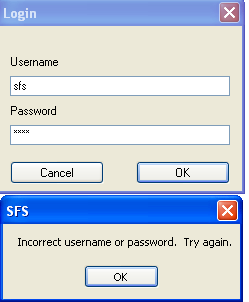
\includegraphics[scale=0.5]{test1dot2scrot}
\caption{The screenshot showing the test 1.2 succeeding.}
\label{fig:test_onedottwo}
\end{figure}

\begin{figure}[ht]
\centering
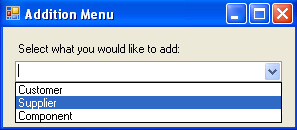
\includegraphics[scale=0.5]{test3dot2scrot}
\caption{The screenshot showing the test 3.2 succeeding.}
\label{fig:test_threedottwo}
\end{figure}

\begin{figure}[ht]
\centering
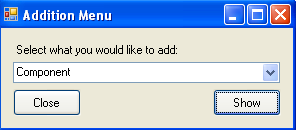
\includegraphics[scale=0.5]{test3dot3scrot1}
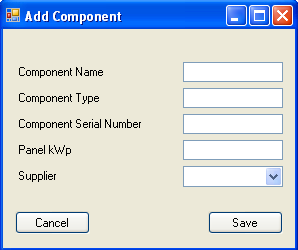
\includegraphics[scale=0.5]{test3dot3scrot2}
\caption{The screenshot showing the test 3.3 succeeding.}
\label{fig:test_threedotthree}
\end{figure}

\begin{figure}[ht]
\centering
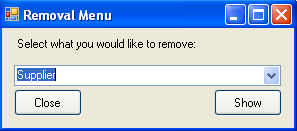
\includegraphics[scale=0.5]{test4dot3scrot1}
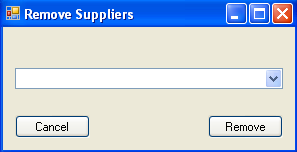
\includegraphics[scale=0.5]{test4dot3scrot2}
\caption{The screenshots showing the test 4.3 succeeding.}
\label{fig:test_fourdotthree}
\end{figure}

\begin{figure}[ht]
\centering
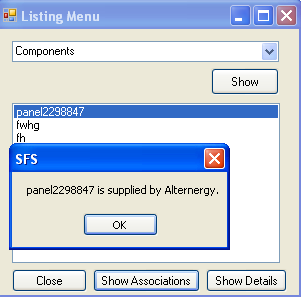
\includegraphics[scale=0.5]{test5dot4scrot}
\caption{Test 5.4 succeeding.}
\label{fig:test_fivedotfour}
\end{figure}

\begin{figure}[ht]
\centering
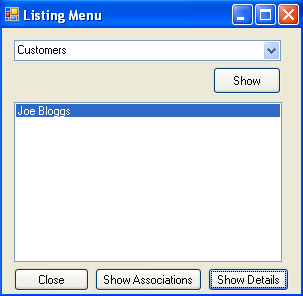
\includegraphics[scale=0.5]{test5dot5scrot1}
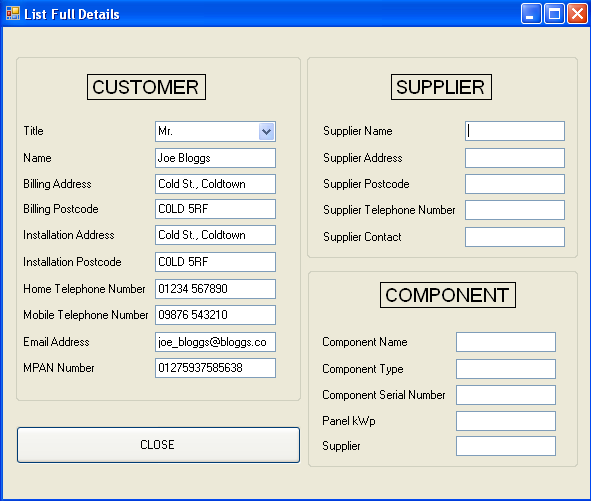
\includegraphics[scale=0.5]{test5dot5scrot2}
\caption{The screenshots showing the test 5.5 succeeding.}
\label{fig:test_fivedotfive}
\end{figure}

\begin{figure}[ht]
\centering
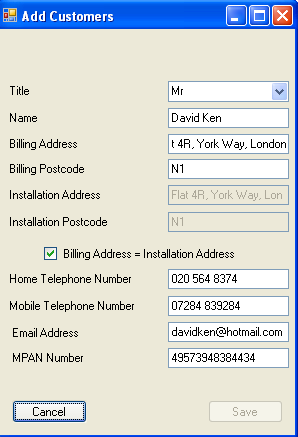
\includegraphics[scale=0.5]{test6dot1scrot1}

\includegraphics[scale=0.5]{test6dot1scrot2}
\caption{The screenshots showing the test 6.1 succeeding.}
\label{fig:test_sixdotone}
\end{figure}

\begin{figure}[ht]
\centering
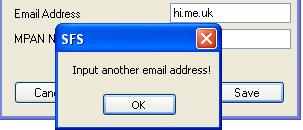
\includegraphics[scale=0.5]{test6dot2scrot}
\caption{The screenshots showing the test 6.2 succeeding.}
\label{fig:test_sixdottwo}
\end{figure}

\begin{figure}[ht]
\centering
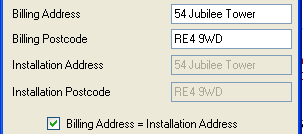
\includegraphics[scale=0.5]{test6dot3scrot1}
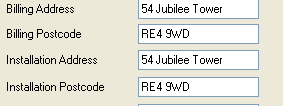
\includegraphics[scale=0.5]{test6dot3scrot2}
\caption{The screenshots showing the test 6.3 succeeding.  The customer details are input in the left screenshot, then obtained from the database in the right screenshot in the List Full Details form.}
\label{fig:test_sixdotthree}
\end{figure}

\begin{figure}[ht]
\centering
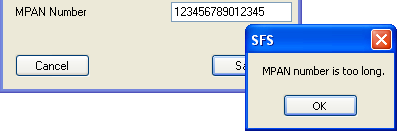
\includegraphics[scale=0.5]{test6dot4}
\caption{The screenshots showing the test 6.4 succeeding.}
\label{fig:test_sixdotfour}
\end{figure}

\begin{figure}[ht]
\centering
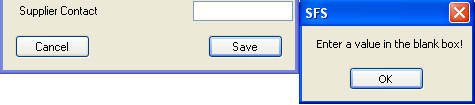
\includegraphics[scale=0.5]{test7dot2}
\caption{The screenshots showing the test 7.2 succeeding.}
\label{fig:test_sevendottwo}
\end{figure}

\begin{figure}[ht]
\centering
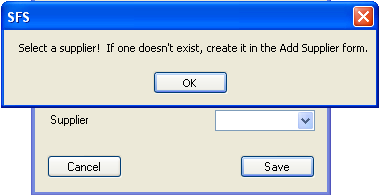
\includegraphics[scale=0.5]{test8dot2}
\caption{The screenshots showing the test 8.2 succeeding.}
\label{fig:test_eightdottwo}
\end{figure}

\begin{figure}[ht]
\centering
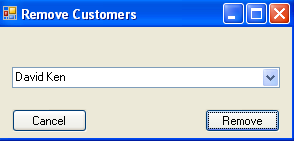
\includegraphics[scale=0.5]{test9dot1scrot1}
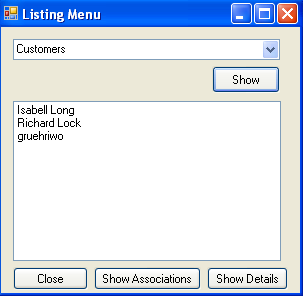
\includegraphics[scale=0.5]{test9dot1scrot2}
\caption{The screenshots showing the test 9.1 succeeding.}
\label{fig:test_ninedotone}
\end{figure}

\begin{figure}[ht]
\centering
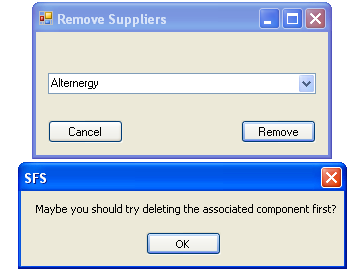
\includegraphics[scale=0.5]{test9dot2}
\caption{The screenshot showing the test 9.2 displaying an error message because the supplier has components associated with it.}
\label{fig:test_ninedottwo}
\end{figure}

\begin{figure}[ht]
\centering
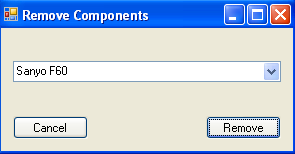
\includegraphics[scale=0.5]{test9dot3scrot1}
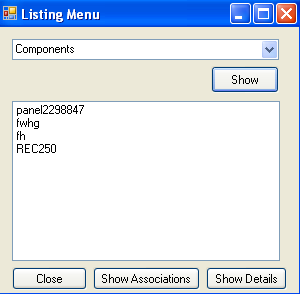
\includegraphics[scale=0.5]{test9dot3scrot2}
\caption{The screenshots showing the test 9.3 succeeding.}
\label{fig:test_ninedotthree}
\end{figure}

\begin{figure}[ht]
\centering
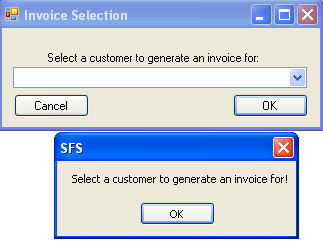
\includegraphics[scale=0.5]{test10dot1}
\caption{The screenshots showing the test 10.1 succeeding.}
\label{fig:test_tendotone}
\end{figure}

\begin{figure}[ht]
\centering
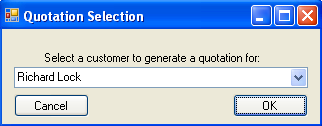
\includegraphics[scale=0.5]{test11dot2scrot1}
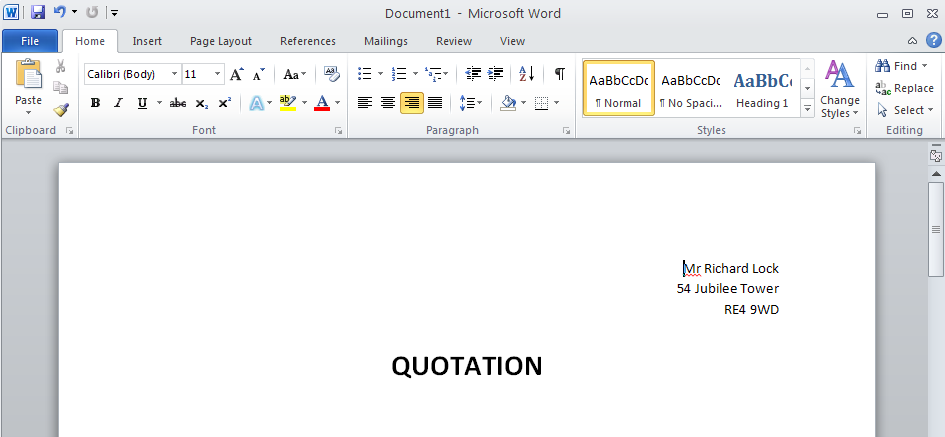
\includegraphics[scale=0.5]{test11dot2scrot2}
\caption{The screenshots showing the test 11.2 succeeding.}
\label{fig:test_elevendottwo}
\end{figure}

\begin{figure}[ht]
\centering
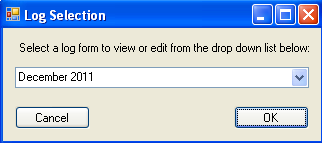
\includegraphics[scale=0.5]{test12dot3scrot1}
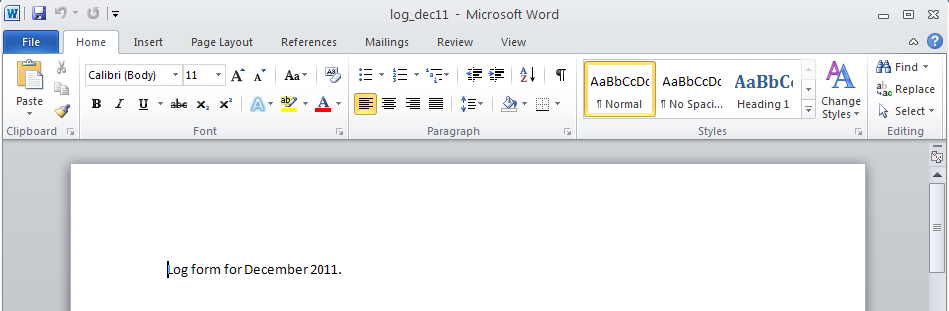
\includegraphics[scale=0.5]{test12dot3scrot2}
\caption{The screenshots showing the test 12.3 succeeding.}
\label{fig:test_twelvedotthree}
\end{figure}